\section{Gramática livre de contexto e Linguagens}

\textbf{Definição:} Uma gramática livre de contexto (GLC) é uma quadra GLC $= (V, \Sigma, P, S)$:

\begin{itemize}
  \item $V =$ é o conjunto \underline{finito} de variáveis;
  \item $\Sigma =$ é o conjunto finito de símbolos terminais (o alfabeto);
  \item $P = $ é o conjunto finito de regras;
  \item $S = $ é o símbolo de partida e $S \in V$
  \item[] $\empty$
  \item[] \textbf{OBS :} $ V \cap \Sigma = \emptyset$
\end{itemize}

\textbf{Características:}

\begin{itemize}
  \item Uma regra, ou produção, é um elemento de $V \times (V \cup \Sigma)^{*}$
  \item $[A, w]$ é escrito como $A \rightarrow w$ (Diz-se que é uma ``Regra A'');
  \item $ \lambda \in (V \cup \Sigma)^{*}$, logo, $ A \rightarrow \lambda $ (Existe e é chamada ``regra lambda'').
\end{itemize}

\textbf{Notação}:\\

\begin{itemize}
  \item \textbf{Minúsculas:} \underline{Terminais}: $(a, b, c, d, e, \ldots)$
  \item \textbf{Maiúsculas:} \underline{Variáveis}: $(A, B, C, D, E, \ldots)$
  \item \textbf{Strings:} \underline{strings}: $p, q, u, v, w, y, x, z$
\end{itemize}

Suponha uma variável $A$ em $uAv$. $A$ aplicação de $A \rightarrow w$ em $uAv$, produz: $uwv$.

Notação:\\
%\begin{center}
\[
uAv \Rightarrow uwv
\]
%\end{center}

\begin{center}
$u$ é o {\color{red} \textbf{prefixo}} e define o {\color{red}\textbf{contexto}}.
\end{center}

Definição (informal): $w$ é \underline{derivável} de $v$ se existe uma sequência finita de aplicações de regras que trasnformam $v$ em $w$, isto é: \\

%\begin{center}
\[
v \Rightarrow w_1 \Rightarrow  w_2 \Rightarrow  \ldots w_n \Rightarrow w
\]
%\end{center}
\textbf{Notação:}\\
%\begin{center}
\[
{\color{red} v \xRightarrow[]{*} w } \\
\]
%\end{center}
%\end{center}


Seja $G = (V, \Sigma, P, S)$ uma GLC, e $v \in (V \cup \Sigma)^{*}$. O conjunto de palavras {\underline{deriváveis de $v$}} é assim definido:\\

\begin{enumerate}
 \item BASE: $v$ é deriváveĺ de $v$;
 \item PASSO RECURSIVO:\\
	SE $u = xAy$ é derivável de $v$\\
	E $A \rightarrow w \in P$, ENTÃO\\
	$xwy$ é derivável de $v$.
  \item FECHO: Apenas as palavras construídas a partir de $v$ por um $n^{o}$ finito de aplicações do passo recursivo são deriváveis a partir de $v$. \\
\end{enumerate}

\underline{Observação}: \\

\begin{itemize}
 \item[] $\rightarrow$: notação para a regra, que é uma relação sobre $Vx(V \cup \Sigma)^{*}$ .
 \item[]$\Rightarrow$ : notação para aplicação de regra, transforma uma sring em outra.
 \item[]$\xRightarrow[]{+}$ : aplicação de uma ou mais vezes a regra.  % $\xRightarrow[world]{hello}$
 \item[]$u \xRightarrow[]{n} w$ : derivação de tamanhoa $n$, isto é, que usou $n$ aplicações de regra.
 \item[]$u \xRightarrow[G]{*} w$ : derivação usando $\empty$ ou mais regras, usando a gramática $G$.
\end{itemize}

\textbf{Definição}:\\

Seja $G = (V, \Sigma, P, S)$ uma GLC:
\begin{enumerate}
  \item Uma palavra $w \in (V \cup \Sigma)^{*}$ é uma {\color{red}forma sentencial} de $G$ se existe uma derivação $S \xRightarrow[G]{*} w$.
  \item Uma \textit{string} $w \in \Sigma^{*}$ é uma {\color{red}sentença} de $G$ se existe uma derivação:\\
  $S \xRightarrow[G]{\ast} w$.
  \item A {\color{red} Linguagem de $G$}, $L(G)$, é o conjunto $\{ w \in \Sigma^{*} | S \xRightarrow[G]{*} w \}$.
\end{enumerate}

\textbf{Definição}:\\
Um conjunto de palavras sobre um alfabeto $\Sigma$ é chamado uma {\color{red}LINGUAGEM LIVRE DE CONTEXTO} se existe uma G.L.C. que a gere.

\begin{itemize}
  \item Uma regra da forma:
    \[
      A \rightarrow uAv
    \]
    é chamada {\color{red}diretamente recursiva}.
  \item Uma variável $A$ é chamada \underline{recursiva} se existe uma derivação:
    \[
      A \xRightarrow{+} uAv
    \]
  \item Uma derivação do tipo
    \begin{center}
      $A \rightarrow w \xRightarrow{+} uAv$, onde $A$ não aparece em $w$\\
      é chamada: {\color{red}INDIRETAMENTE RECURSIVA}.
    \end{center}
\end{itemize}

\underline{Exemplo}: \\

Linguagem $L$ das palavras sobre $\{a,b\}$, que tem um $n^{o}$ par de $a's$:\\
\begin{itemize}
 \item[] $G = (V, \Sigma, P, S)$
 \item[] $V = \{S,A\}$
 \item[] $\Sigma = \{a,b\}$
 \item[] $P:$\\
    \begin{itemize}
     \item[] $S \rightarrow$ AA
     \item[] $A \rightarrow$ AAA | \texttt{b}A | \texttt{A}b | \texttt{a}
    \end{itemize}
\end{itemize}

Derivações de \underline{\texttt{ababaa}}: \\

\begin{center}
\begin{tabular}{l | l | l | l}
$S \Rightarrow$ AA 		                & $S \Rightarrow$ AA 		              & $S \Rightarrow$ AA 			                     & $S \Rightarrow$ AA\\
$\quad \Rightarrow$ \texttt{a}A 	    & $\quad \Rightarrow$ AAAA 		        & $\quad \Rightarrow$ A\texttt{a}  		         & $\quad \Rightarrow$ \texttt{a}A\\
$\quad  \Rightarrow$ \texttt{ab}AAA 	& $\quad \Rightarrow$ \texttt{a}AAA 	& $\quad \Rightarrow$ AAA\texttt{a} 	         & $\quad \Rightarrow$ \texttt{a}AAA\\
$\quad  \Rightarrow$ \texttt{ab}AAA 	& $\quad \Rightarrow$ \texttt{ab}AAA  & $\quad \Rightarrow$ AA\texttt{b}A\texttt{a}  & $\quad \Rightarrow$ \texttt{a}AA\texttt{a}\\
$\quad  \Rightarrow$ \texttt{aba}AA 	& $\quad \Rightarrow$ \texttt{aba}AA  & $\quad \Rightarrow$ AA\texttt{baa} 	         & $\quad \Rightarrow$ \texttt{ab}AA\texttt{a}\\
$\quad  \Rightarrow$ \texttt{abab}AA 	& $\quad \Rightarrow$ \texttt{abab}AA & $\quad \Rightarrow$ A\texttt{b}A\texttt{baa} & $\quad \Rightarrow$ \texttt{ab}A\texttt{b}A\texttt{a}\\
$\quad  \Rightarrow$ \texttt{ababa}A 	& $\quad \Rightarrow$ \texttt{ababa}A & $\quad \Rightarrow$ A\texttt{babaa} 	       & $\quad \Rightarrow$ \texttt{abab}A\texttt{a}\\
$\quad  \Rightarrow$ \texttt{ababaa} 	& $\quad \Rightarrow$ \texttt{ababaa} & $\quad \Rightarrow$ \texttt{ababaa} 	       & $\quad \Rightarrow$ \texttt{ababaa}
\end{tabular}
\end{center}

\textbf{Obs}:\\

\begin{itemize}
  \item Derivação $(a)$ é chamada {\color{red}``Mais à esquerda''}
  \item Derivação $(c)$ é chamada {\color{red}``Mais à direita''}
\end{itemize}

\textbf{Definição}:\\

Seja $G = (V, \Sigma, P, S)$ uma GLC, e $S \xRightarrow[G]{*} w$ uma derivação.\\
A {\color{red} árvore de derivação} de $S \xRightarrow[G]{*} w$  é uma \underline{árvore ordenada} (\textbf{AD}) que pode ser assim construída:\\

\begin{enumerate}
  \item[i] Inicialize \textbf{AD} com $S$ na raiz;
  \item[ii] Se $A \rightarrow x_{1}x_{2}\ldots x_{n} (x_{i} \in (V \cup S))$ é uma regra, na derivação aplicada na string $A \rightarrow uAv$, então adicione $x_{1}, x_{2}, \ldots, x_{n}$ como filhos de $A$ na árvore;
  \item[iii] Se $A \rightarrow \lambda$ é uma regra na derivação aplicada na string $uAv$, adicione $\lambda$ como único filho de $A$ na árvore.
\end{enumerate}

\begin{center}
\begin{longtable}{l  c  c }
%   \toprule
  Derivação & Árvore & Ordenação \\
 \hline
%  \toprule
 % segunda linha
  {\color{blue}S}                 & S & {\color{red} S}\\
 % terceira linha
  {\color{blue}$ \Rightarrow$ AA} & \begin{tikzpicture}[level distance=1cm]
  \node {S}
  child {node {A}}
  child {node {A}};
 \end{tikzpicture} & {\color{red} A,A}\\
 % quarta linha
 {\color{blue}$ \Rightarrow$ a} & \begin{tikzpicture}[level distance=1cm]
 \node {S}
 child {node {A}
  child {node {\texttt{a}}}}
  child {node {A}};
  \end{tikzpicture} & {\color{red} a,A}\\
  % quinta linha
  {\color{blue}$ \Rightarrow$ aAAA} & 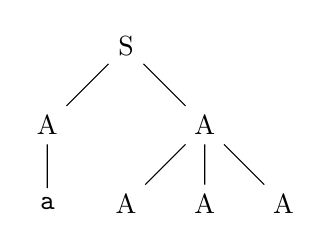
\begin{tikzpicture}[level distance=1cm]
  \tikzstyle{level 1}=[sibling distance=2cm]
  \tikzstyle{level 2}=[sibling distance=1cm]
  \node {S}
  child {node {A}
    child {node {\texttt{a}}}}
  child {node {A}
    child {node {A}}
    child {node {A}}
    child {node {A}}};
  \end{tikzpicture} & {\color{red} a,A,A,A}\\
  % sexta linha
  {\color{blue}$ \Rightarrow$ abAAA} & 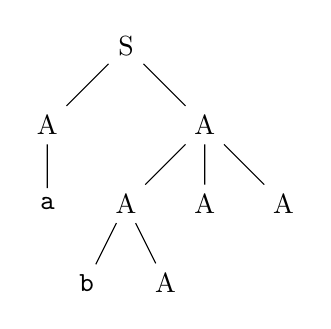
\begin{tikzpicture}[level distance=1cm]
  \tikzstyle{level 1}=[sibling distance=2cm]
  \tikzstyle{level 2}=[sibling distance=1cm]
  \node {S}
  child {node {A}
    child {node {\texttt{a}}}}
  child {node {A}
    child {node {A}
    child {node {\texttt{b}}}
    child {node {A}}}
    child {node {A}}
    child {node {A}}};
  \end{tikzpicture} & {\color{red} a,b,A,A,A}\\
  % sétima linha
  {\color{blue}$ \Rightarrow$ abaAA} & \begin{tikzpicture}[level distance=1cm]
  \tikzstyle{level 1}=[sibling distance=2cm]
  \tikzstyle{level 2}=[sibling distance=1cm]
  \node {S}
  child {node {A}
    child {node {\texttt{a}}}}
  child {node {A}
    child {node {A}
    child {node {\texttt{b}}}
    child {node {A}
    child {node {\texttt{a}}}}}
    child {node {A}}
    child {node {A}}};
  \end{tikzpicture} & {\color{red} a,b,a,A,A}\\
  % oitava linha
  {\color{blue}$ \Rightarrow$ ababAA} & \begin{tikzpicture}[level distance=1cm]
  \tikzstyle{level 1}=[sibling distance=4cm]
  \tikzstyle{level 2}=[sibling distance=2cm]
  \tikzstyle{level 3}=[sibling distance=1cm]
  \node {S}
  child {node {A}
    child {node {\texttt{a}}}}
  child {node {A}
    child {node {A}
    child {node {\texttt{b}}}
    child {node {A}
    child {node {\texttt{a}}}}}
    child {node {A}
    child {node {\texttt{b}}}
    child {node {A}}}
    child {node {A}}};
  \end{tikzpicture} & {\color{red} a,b,a,b,A,A}\\
  % nona linha
  {\color{blue}$ \Rightarrow$ ababaA} & \begin{tikzpicture}[level distance=1cm]
  \tikzstyle{level 1}=[sibling distance=4cm]
  \tikzstyle{level 2}=[sibling distance=2cm]
  \tikzstyle{level 3}=[sibling distance=1cm]
  \node {S}
  child {node {A}
    child {node {\texttt{a}}}}
  child {node {A}
    child {node {A}
    child {node {\texttt{b}}}
    child {node {A}
    child {node {\texttt{a}}}}}
    child {node {A}
    child {node {\texttt{b}}}
    child {node {A}
    child {node {\texttt{a}}}}}
    child {node {A}}};
  \end{tikzpicture} & {\color{red} a,b,a,b,a,A}\\
  % décima linha
  {\color{blue}$ \Rightarrow$ ababaa} & \begin{tikzpicture}[level distance=1cm]
  \tikzstyle{level 1}=[sibling distance=4cm]
  \tikzstyle{level 2}=[sibling distance=2cm]
  \tikzstyle{level 3}=[sibling distance=1cm]
  \node {S}
  child {node {A}
    child[red] {node {\texttt{a}}}
  }
  child {node {A}
    child {node {A}
      child[red] {node {\texttt{b}}}
      child {node {A}
      child[red] {node {\texttt{a}}}
      }
    }
    child {node {A}
      child[red] {node {\texttt{b}}}
      child {node {A}
        child[red] {node {\texttt{a}}}
      }
    }
    child {node {A}
      child[red] {node {\texttt{a}}}
    }
  };
  \end{tikzpicture}  & {\color{red} a,b,a,b,a,a}
%fim
\end{longtable}
\end{center}

\textbf{Ordenação}: {\color{red}(Para obtermos o resultado da derivação)}\\

\begin{enumerate}
  \item Inicialmente: a única folha é $S$ e a ordenação é óbvia.
  \item Quando uma regra $A \rightarrow x_{1}x_{2}\ldots x_{n} (x_{i}$ é aplicada para gerar os filhos de $A$, cada $x_{i}$ se torna uma folha e $A$ é substituída na ordenação das folhas pela sequência $x_{1}, x_{2}, \ldots, x_{n}$.
  \item A aplicação da regra $A \rightarrow \lambda$ provoca a simples troca de $A$ pela palavra vazia.
\end{enumerate}

\begin{center}
  A {\color{red}Fronteira} da árvore de derivação é a palavra gerada pela derivação.
\end{center}

\begin{center}
\begin{tabular}{c  c }
 % primeira linha, primeira coluna
 % a
 \begin{tikzpicture}[level distance=1cm]
  \tikzstyle{level 1}=[sibling distance=4cm]
  \tikzstyle{level 2}=[sibling distance=2cm]
  \tikzstyle{level 3}=[sibling distance=1cm]
   \node {S}
    child {node {A}
     child[blue] {node {\texttt{a}}}
    }
    child {node {A}
     child {node {A}
       child[blue] {node {\texttt{b}}}
       child {node {A}
       child[blue] {node {\texttt{a}}}
       }
     }
     child {node {A}
       child[blue] {node {\texttt{b}}}
       child {node {A}
         child[blue] {node {\texttt{a}}}
       }
     }
     child {node {A}
       child[blue] {node {\texttt{a}}}
     }
    };
   \end{tikzpicture} &
 % primeira linha, segunda coluna
 % b
 \begin{tikzpicture}[level distance=1cm]
   \tikzstyle{level 1}=[sibling distance=4cm]
   \tikzstyle{level 2}=[sibling distance=2cm]
   \tikzstyle{level 3}=[sibling distance=1cm]
   \node {S}
    child {node {A}
    child {node {A}
      child[red] {node {\texttt{a}}}
    }
     child {node {A}
       child[red] {node {\texttt{b}}}
       child {node {A}
       child[red] {node {\texttt{a}}}
       }
     }
     child {node {A}
       child[red] {node {\texttt{b}}}
       child {node {A}
         child[red] {node {\texttt{a}}}
       }
     }
    }
    child {node {A}
     child[red] {node {\texttt{a}}}
    };
 \end{tikzpicture}\\
 % linha so pras legendas
 {\color{blue}$(a)$} & {\color{red}$(b)$}\\
 % segunda linha, primeira coluna
 % d
 \begin{tikzpicture}[level distance=1cm]
 \tikzstyle{level 1}=[sibling distance=4cm]
 \tikzstyle{level 2}=[sibling distance=2cm]
 \tikzstyle{level 3}=[sibling distance=1cm]
 \node {S}
  child {node {A}
   child[blue] {node {\texttt{a}}}
  }
  child {node {A}
   child {node {A}
     child[blue] {node {\texttt{b}}}
     child {node {A}
     child[blue] {node {\texttt{a}}}
     }
   }
   child {node {A}
     child[blue] {node {\texttt{b}}}
     child {node {A}
       child[blue] {node {\texttt{a}}}
     }
   }
   child {node {A}
     child[blue] {node {\texttt{a}}}
   }
  };
 \end{tikzpicture} &
 \begin{tikzpicture}[level distance=1cm]
   \tikzstyle{level 1}=[sibling distance=4cm]
   \tikzstyle{level 2}=[sibling distance=2cm]
   \tikzstyle{level 3}=[sibling distance=1cm]
   \node {S}
    child {node {A}
    child {node {A}
      child[red] {node {\texttt{a}}}
    }
     child {node {A}
       child[red] {node {\texttt{b}}}
       child {node {A}
       child[red] {node {\texttt{a}}}
       }
     }
     child {node {A}
       child[red] {node {\texttt{b}}}
       child {node {A}
         child[red] {node {\texttt{a}}}
       }
     }
    }
    child {node {A}
     child[red] {node {\texttt{a}}}
    };
 \end{tikzpicture}\\
 % linha so pras legendas
 {\color{blue}$(d)$} & {\color{red}$(c)$}\\
  %fim
\end{tabular}
\end{center}

\textbf{Observações}:\\

\begin{itemize}
  \item Pode-se reconstruir as derivações a partir da árvore de derivação.
  \item A liberdade de aplicação das regras {\color{red}(livre de contexto)} permite grande flexibilidade na construção das derivações, além de modularidade.
  \item Esta modularidade é explorada no desenvolvimento de linguagens complexas.
  \item Ao aluno interessado na prova formal destes comentários, indicamos a página 65 do livro base do curso (Sudkamp) {\color{red} Veja Lema 3.1.5}
\end{itemize}

